In the previous section each component of the system was modeled with differential and algebraic equations. The modeling format is such that every component takes some inputs, and from those calculates some states and some outputs which are used for the adjacent components. In order to make a complete non-linear model it is necessary to connect the inputs and outputs of the system. This section provides insight into how components are interfaced and collected into a complete non-linear state space form.

A block diagram is made to give an overview of the system interface variables and states. All differential equations are states of the system and they are collected in a vector $f(x,u)$ where $u$ encapsulates both the controlled and uncontrolled inputs (disturbances). The algebraic constraint equations are substituted into the state vector variables until the state derivatives are functions only of states, inputs and disturbances.\\

In \cref{fig:Block_diagram_inout} the component interface variables are split out to show which variables are used as inputs and outputs for each component. Some inputs to components are highlighted in red to signify that they are not found as outputs from a component. Steady State values (operating points) for these are found from the Hi-Fi simulation and used. Blue variables are outputs of components which are currently not used by the following component. Each component block also contains the names of the states they contain.

\begin{figure}[h!]
	\centering
	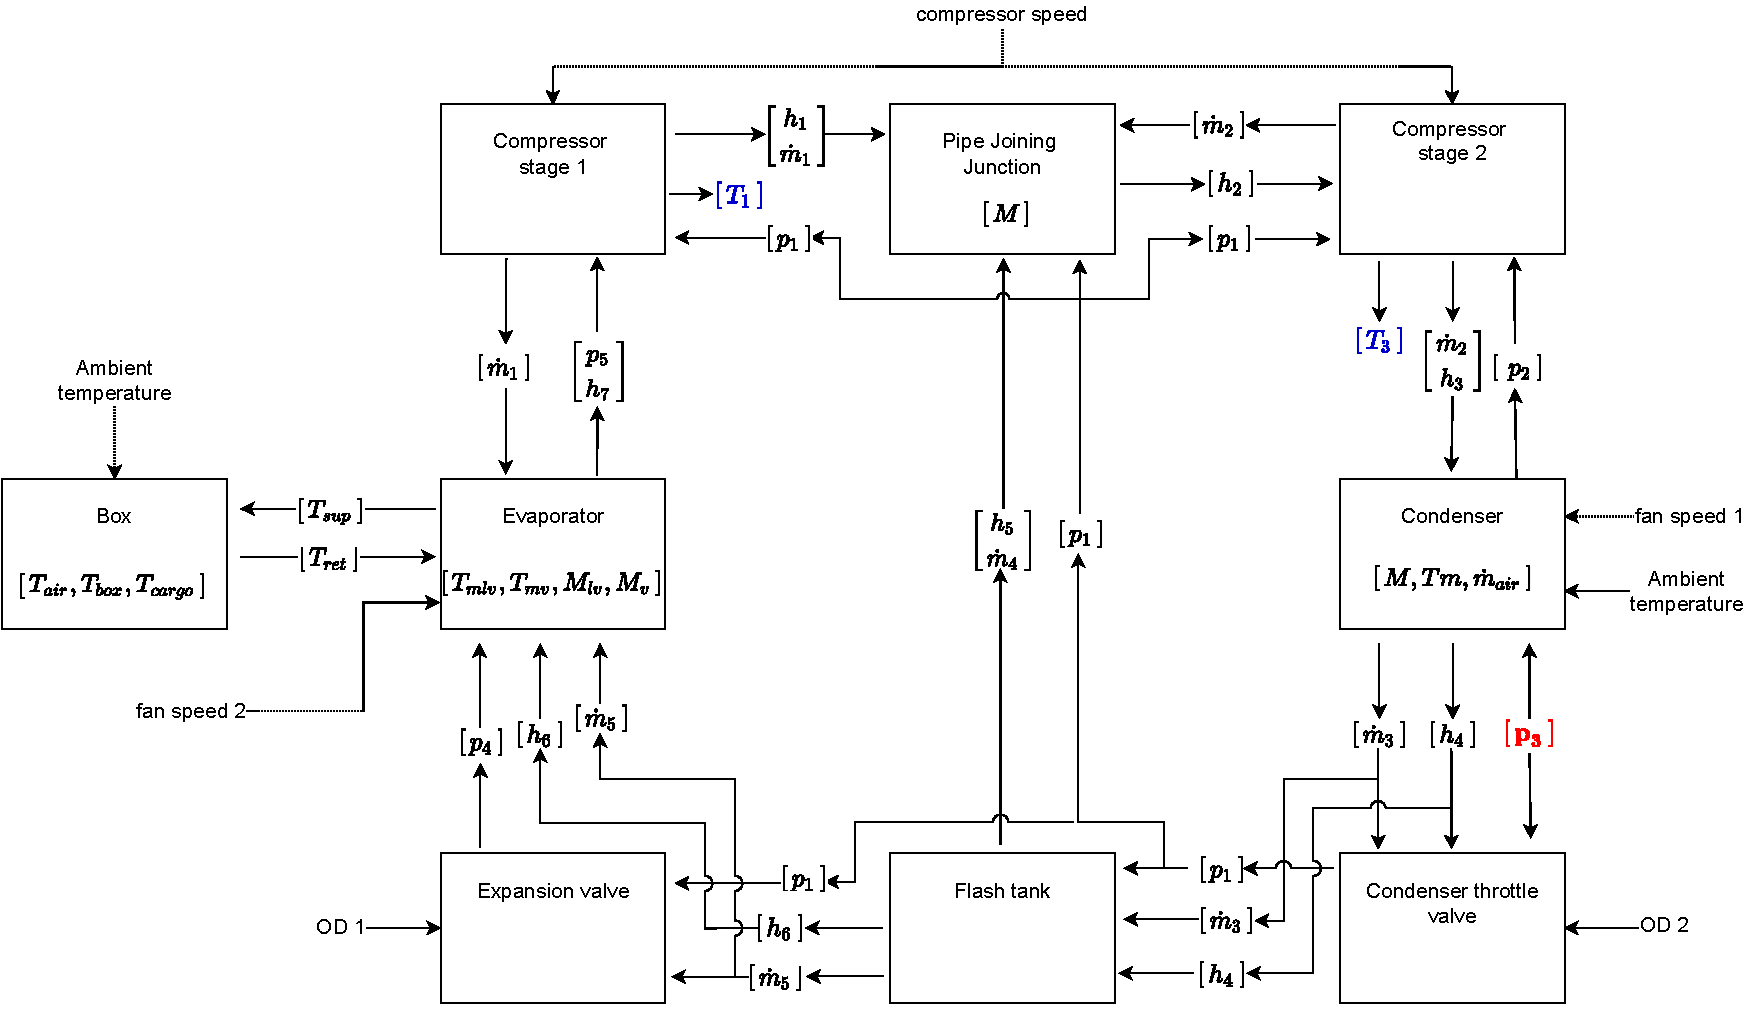
\includegraphics[width=1\textwidth]{Graphics/Block_Diagram_inout.pdf}
	\caption{Block diagram of input/output relationship of interface variables}
	\label{fig:Block_diagram_inout}
\end{figure}


\newpage

\subsubsection{State variables}

Due to the large variance in the dynamic speed of the system parameters, the fast variables were defined algebraically, while the slow dynamics were modeled with differential equations. This is possible because the fast variables settle to steady state values without oscillatory behavior. \\

While including the dynamics of the faster parameters would yield a potentially more accurate model, it is unnecessary from a control perspective, as this model is intended for control of the slow dynamics. In addition, the added accuracy will likely be unnoticeable due to various uncertainties in the model. The specific decision of which parameters to model dynamically is heavily inspired by previous work \cite{Sorensen2013}.

The differential equations are collected in the state vector in \cref{eq:f_noSub}.


% F: States
% ------------------------------------

\begin{equation} \label{eq:f_noSub} \renewcommand{\arraystretch}{2.4}
	f(x,u) =  \dfrac{d}{dt} \begin{bmatrix}
		M_{pjj}			\\				%pjj
		M_{con} 		\\				%condenser
		T_m 			\\				%condenser
		\dot{m}_{air}	\\				%evaporator
		T_{mlv}			\\				%evaporator
		T_{mv}			\\				%evaporator
		M_{lv}			\\				%evaporator
		M_v				\\				%evaporator
		T_{air}			\\				%box
		T_{box}			\\				%box
		T_{cargo}		\\				%box

	\end{bmatrix}
	=
	\begin{bmatrix}
		\dot{m}_1 + \dot{m}_4 - \dot{m}_2 \\										%pjj
		\dot{m}_{2} - \dot{m}_{3}	\\												%condenser
		\dfrac{Q_{rm} - Q_{ma}}{M_m \cdot Cp_m} \\									%condenser
		\dfrac{\bar{\dot{m}}_{air}  - \dot{m}_{air}} {10s}		\\					%evaporator
		\dfrac{Q_{aml}-Q_{ml} + Q_{mvml}}{M_m \cdot Cp_m \cdot \sigma}        \\	%evaporator
		\dfrac{Q_{amv} - Q_{mv} - Q_{mvml}}{M_m \cdot Cp_m \cdot (1- \sigma)}	\\	%evaporator
		\dot{m}_{5} - \dot{m}_{dew}		\\											%evaporator
		\dot{m}_{dew} - \dot{m}_{1}	\\												%evaporator
		\dfrac{Q_{ca} + Q_{ba} + Q_{fan} -Q_{cool}}{M_{air} \cdot Cp_{air}} \\		%box
		\dfrac{Q_{amb} - Q_{ba}}{M_{box} \cdot Cp_{box}} \\							%box
		\dfrac{-Q_{ca}}{M_{cargo} \cdot Cp_{cargo}}									%box
	\end{bmatrix}
\end{equation}


As mentioned all variables which are not states, inputs and disturbances in \cref{eq:f_noSub} are substituted with the algebraic equations. As such the states, inputs and disturbances are included in the state derivatives. The function $f(x,u)$ is thus the non-linear model of the system. Writing out the full state space system is infeasible due to the sheer size of expressions when substitution is performed. The model contains 11 states, 5 control inputs and 1 disturbance.

The control inputs are:

\begin{center}
	\begin{tabular}{l p{10cm}}
		$ \Theta_1 $  & The valve opening degree of the \\
		$ \Theta_2 $  & The valve opening degree of the \\
		$ U_{fan_1} $ & The condenser fan speed         \\
		$ U_{fan_2} $ & The evaporator fan speed        \\
		$ \omega $    & The compressor speed
	\end{tabular}
\end{center}

The disturbance is:

\begin{center}
	\begin{tabular}{l p{10cm}}
		$ T_{ambi} $  & The ambient air temperature
	\end{tabular}
\end{center}